% ============================================================
%  深圳大学实验报告模板（SZU Experiment Report Template）
% This template can be modified according to the specific requirements of your experiment or project.
% Produced by: Chao Fan and Kewei Ou, AI School of SZU
% ============================================================

\documentclass[a4paper,12pt]{article}

% ----------------------------
% 中文与字体支持
% ----------------------------
\usepackage{fontspec}    % 字体支持
\usepackage{xeCJK}       % 中文字体支持
\setCJKmainfont{Noto Serif CJK SC} % 设置中文字体（Overleaf自带Noto字体）

% ----------------------------
% 页面设置与常用宏包
% ----------------------------
\usepackage{geometry}    % 页面边距控制
\geometry{left=1in, right=1in, top=1in, bottom=1in}

\usepackage{longtable}   % 支持长表格
\usepackage{graphicx}    % 插入图片
\usepackage{fancyhdr}    % 页眉页脚控制
\usepackage{tikz}        % 绘制框线等图形
\usetikzlibrary{calc}    % 坐标计算
\usepackage{verbatim}    % 显示代码块
\usepackage{float}       % 控制图片浮动位置（[H]参数）
\usepackage{url}         % 网址断行

% ----------------------------
% 页眉页脚设置
% ----------------------------
% \pagestyle{fancy}
\fancyhf{} % 清空默认页眉页脚
% \fancyhead[L]{深圳大学实验报告} % 左侧页眉文字
\fancyhead[C]{} % 中间空
\fancyhead[R]{} % 右侧空

% ============================================================
%                      文档开始
% ============================================================

\begin{document}

% ============================================================
% 封面页
% ============================================================
\begin{titlepage}
    \centering
    \vspace*{2cm}
    \Huge{\textbf{深 \ 圳 \ 大 \ 学 \ 实 \ 验  \ 报 告}}\\[1.5cm]
    
    {\Large\textbf{课程名称}\quad\underline{\makebox[8cm][c]{Python程序设计}}}\\[0.5cm]
{\Large
\noindent\makebox[3.2cm][l]{\textbf{项目名称}}
\underline{\makebox[8cm][c]{ViT-B/32 图像编码器的 NumPy 复现}}}\\[0.5cm]
{\Large
\noindent\makebox[3.2cm][l]{\textbf{学 \quad \quad 院}}
\underline{\makebox[8cm][c]{人工智能学院}}}\\[0.5cm]
{\Large
\noindent\makebox[3.2cm][l]{\textbf{专 \quad \quad 业}}
\underline{\makebox[8cm][c]{人工智能}}}\\[0.5cm]
{\Large
\noindent\makebox[3.2cm][l]{\textbf{指导教师}}
\underline{\makebox[8cm][c]{舒婷}}}\\[0.5cm]
{\Large
\noindent\makebox[3.2cm][l]{\textbf{报 \quad 告 \quad 人}}
\underline{\makebox[3cm][c]{彭佳琦}}
\hspace{0.5cm}
\textbf{学号}
\underline{\makebox[3cm][c]{2025681109}}}\\[0.5cm]
{\Large
\noindent\makebox[3.2cm][l]{\textbf{实验时间}}
\underline{\makebox[8cm][c]{2026 年 11 月 20 日 -- 11 月 26 日}}}\\[0.5cm]
{\Large
\noindent\makebox[3.2cm][l]{\textbf{提交时间}}
\underline{\makebox[8cm][c]{2026 年 11 月 27 日}}}\\[1.5cm]

    \vfill
    \Large{\textbf{教务处制}}
\end{titlepage}

\newpage

% ============================================================
% 正文部分
% ============================================================
% Experiment Objectives


\section{Objectives}

本项目要求在不使用 PyTorch 等深度学习框架的前提下，仅用 NumPy 补全课程给定的 OpenCLIP ViT-B/32 视觉编码器，使其前向计算结果与课程提供的独立 Torch FP32 参考在数值上一致。输入是预处理后的图像批次 $[B,3,224,224]$（float32），输出是每张图一个 512 维单位向量 $[B,512]$，也即期末项目 szu\_python\_openclip 图像塔的最终输出。

数据为课程附件中的 10 张真实图片（短边缩放 + 中心裁剪到 $224\times224$，按 OpenCLIP 的均值与标准差归一化）以及 152 个 visual.* 参数张量，共 87{,}849{,}216 个 float32 值。全程只做前向推理，不含任何训练或参数更新，因此本任务考察的是对数组轴、形状变换与矩阵乘法的掌握。判定标准为：形状一致、dtype 为 float32、全部有限，且 $|y-\hat{y}|\le \mathrm{atol}+\mathrm{rtol}\,|\hat{y}|$，其中预处理 atol 为 $2\times10^{-6}$、内部 token 为 $2\times10^{-4}$、最终输出为 $2\times10^{-5}$，rtol 统一取 $2\times10^{-4}$。交付物包括实现代码、说明功能与结构的 README（含依赖清单与权重获取方式）、8 条以上的分步提交记录，以及本实验报告；权重文件（326 MB）与参考输出按课程要求不入库，README 中给出两者的 SHA-256 校验值。

\noindent 代码仓库：\url{https://github.com/PJQpjq1218/project1-vit-b32-numpy}（README 说明项目功能与结构、依赖清单、数据获取方法与复现步骤）


% Experiment Process
\section{Overview}
整条管线分为五步：

\begin{enumerate}
    \item[Step 1]: patchify，把 $[B,3,224,224]$ 切成 49 个 $32\times32$ 的块，块间按「先左右、后上下」编号，块内按 $C,H,W$ 展平，得到 $[B,49,3072]$；
    \item[Step 2]: embed，无偏置的块线性投影得到 $[B,49,768]$，拼接可学习的 CLS 行并加上位置编码，得到 $[B,50,768]$；
    \item[Step 3]: 12 层 Pre-LN TransformerBlock，每层为「LN + 12 头注意力 + 残差」再「LN + MLP + 残差」，形状始终保持 $[B,50,768]$；
    \item[Step 4]: 输出头，取 CLS 行，经 ln\_post 与 $768\times512$ 投影得到 $[B,512]$；
    \item[Step 5]: 逐行 L2 归一化，使每个输出 token 的模长为 1。
\end{enumerate}

预处理由课程提供：短边缩放到 224、中心裁剪，再按 OpenCLIP 的均值 $[0.48145,0.45783,0.40821]$ 与标准差 $[0.26863,0.26130,0.27578]$ 逐通道归一化，因此本节所有形状都从 $[B,3,224,224]$ 开始。

核心计算如式 (1)、(2) 所示，其中 $Q=XW_q^{\top}+b_q$，三个投影由一次 $[B,50,2304]$ 的合并矩阵乘得到后按 12 个头切分，GELU 采用精确的 $\mathrm{erf}$ 形式 $0.5u\,(1+\mathrm{erf}(u/\sqrt{2}))$：

\begin{equation}
\mathrm{LN}(x)=\frac{x-\mu}{\sqrt{\sigma^2+10^{-5}}}\odot\gamma+\beta,
\qquad
A=\mathrm{softmax}\!\left(\frac{QK^{\top}}{\sqrt{64}}\right)V
\end{equation}
\begin{equation}
X_1=X+AW_o^{\top}+b_o,
\qquad
X_2=X_1+\mathrm{GELU}(X_1W_1^{\top}+b_1)\,W_2^{\top}+b_2
\end{equation}

图~\ref{fig:vit-arch} 给出图像塔结构与本文复现的数据流，表~\ref{tab:shapes} 列出各阶段的数组形状。

% Figure
\begin{figure}[H]
    \centering
    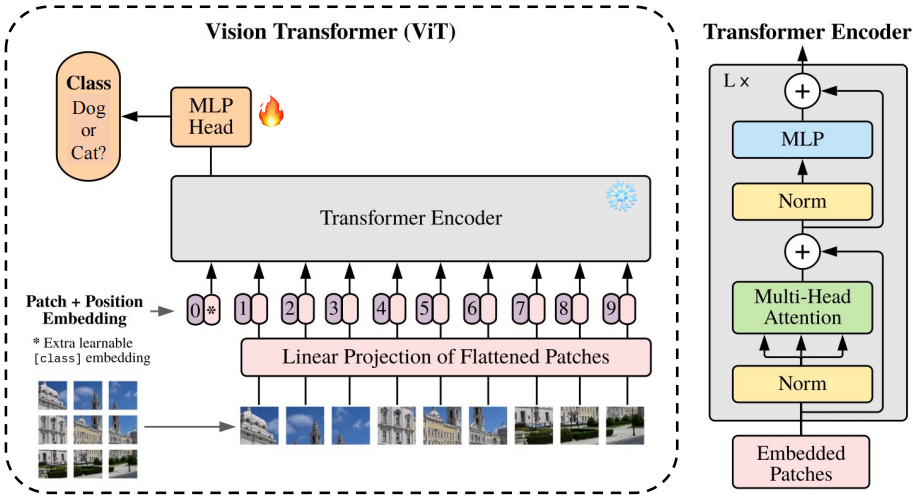
\includegraphics[width=0.86\linewidth]{figs/vit_overview.png}
    \caption{ViT-B/32 图像塔结构与本文复现的计算路径（$B$ 为批量大小）}
    \label{fig:vit-arch}
\end{figure}

\begin{table}[H]
    \centering
    \small
    \begin{tabular}{|p{2.5cm}|p{3.1cm}|p{8.3cm}|}
    \hline
    阶段 & 数组形状 & 关键算子 \\
    \hline
    预处理输入 & $[B,3,224,224]$ & BICUBIC 缩放、中心裁剪、按 OpenCLIP 均值方差归一化 \\
    \hline
    patchify & $[B,49,3072]$ & reshape $\to$ transpose $\to$ reshape \\
    \hline
    embed & $[B,50,768]$ & 块投影（无 bias）、拼接 CLS、加位置编码 \\
    \hline
    Q/K/V & $[B,12,50,64]$ & 合并投影后按 12 个头切分 \\
    \hline
    scores & $[B,12,50,50]$ & $QK^{\top}/\sqrt{64}$ 后做 softmax \\
    \hline
    block 输出 & $[B,50,768]$ & 注意力残差 + MLP 残差，共 12 层串联 \\
    \hline
    输出 token & $[B,512]$ & CLS $\to$ ln\_post $\to$ 投影 $\to$ 单位化 \\
    \hline
    \end{tabular}
    \caption{各阶段数组形状与关键算子}
    \label{tab:shapes}
\end{table}

% Implementation Details
\section{Implementations}
需要实现的只有 image\_encoder.py 中的六个 TODO，课程提供的 helpers.py（LN、GELU、softmax、单位化）、preprocess\_image.py、check.py 与 run.py 均未改动。

\begin{enumerate}
    \item[TODO-01]: patchify，用 reshape 把 $H,W$ 各拆成「7 个块位置 + 32 像素」，transpose 把轴重排为「图像、块行、块列、$C$、块内行、块内列」，最后 flatten 成 $[B,49,3072]$；
    \item[TODO-02]: split\_heads，把特征轴 $D$ 按连续 64 维切成 12 段，再换轴得到 $[B,12,N,64]$，token 顺序与头内顺序都不动；
    \item[TODO-03]: 计算 $QK^{\top}/\sqrt{64}$ 的 scores，softmax 后与 $V$ 做加权求和，把头并回特征轴，再做输出投影（权重按 [out,in] 存放，须转置）；
    \item[TODO-04]: 块内两处残差与 MLP，即 $X_1=X+\mathrm{attn}(\mathrm{LN}(x))$ 与 $X_2=X_1+\mathrm{MLP}(\mathrm{LN}(X_1))$；
    \item[TODO-05]: 块投影无 bias，拼接 CLS 后与位置编码广播相加；
    \item[TODO-06]: 取 CLS 行、过 ln\_post、乘 $[768,512]$ 的 visual.proj（该权重已是 [in,out]，不再转置）、最后单位化。
\end{enumerate}

实现中需要特别注意的约定有四条：其一，注意力与 MLP 的线性层权重都按 [out,in] 存放，必须用 $W^{\top}$，只有 visual.proj 是 [in,out]；其二，$k$ 是 4D 张量，只能用 \texttt{transpose(0,1,3,2)} 交换最后两轴，直接用 \texttt{k.T} 会把 batch 与 head 轴一并反转；其三，split\_heads 必须按连续 64 维切分，不能按步长交错取；其四，全程保持 float32，缩放因子写成 \texttt{np.float32(np.sqrt(64))}，避免与 float64 标量运算时被提升精度。

\paragraph{规范与边界处理}
参数只读：所有偏置与权重直接从加载的数组取用，实现中不出现任何原地修改，便于把同一份代码复用到期末项目；入口处校验输入形状，非 $[B,3,224,224]$ 时抛出带具体形状的 \texttt{ValueError}，而不是让后续的 reshape 报出难以定位的错误；对关键中间量（$q,k,v$ 与 scores）在开发期加形状断言，正是这些断言把 4D 转置的错误在 block0 阶段就暴露出来。

\paragraph{代码结构}
三个类分工明确：MultiHeadAttention 负责切头、打分、加权与输出投影；TransformerBlock 组合两处 LN、注意力与 MLP；ImageEncoder 负责 patchify、embed、12 层串联与输出头。公共超参（宽 768、12 头、头维 64、MLP 中间层 3072）全部读自 config.json，代码中不做硬编码假设，因此同一份实现可以直接用于期末项目的图像塔。

\paragraph{本人贡献}
本人独立完成上述六个 TODO 与边界检查（输入非 $[B,3,224,224]$ 时抛出 \texttt{ValueError}），并自行编写了证据脚本（分阶段误差、耗时统计、六组对照实验）与本报告；课程提供的文件一行未改。过程中使用 AI 助手辅助解释 4D 张量的轴语义、复核 reshape/transpose 的轴序与报告排版，所有数值结论均由本机实际运行 \texttt{check.py} 得到并逐项核对。

\section{Results}

在干净环境下执行 \texttt{python check.py --stage all}，八个阶段全部通过，结果见表~\ref{tab:errors} 与图~\ref{fig:err}。patch 与预处理阶段的最大误差严格为 0，说明切块顺序与归一化完全正确；内部 token 的误差在 $10^{-5}$ 量级，仅来自矩阵乘法的累加顺序；最终输出 token 的最大误差为 $5.4\times10^{-7}$，比容差 $2\times10^{-5}$ 小约 37 倍。

\begin{table}[H]
    \centering
    \small
    \begin{tabular}{|p{5.0cm}|p{2.4cm}|p{2.4cm}|p{1.7cm}|p{1.3cm}|}
    \hline
    阶段（形状） & 最大绝对误差 & 平均绝对误差 & atol & 判定 \\
    \hline
    patchify $[2,49,3072]$ & $0$ & $0$ & $2\times10^{-4}$ & PASS \\
    \hline
    embed $[2,50,768]$ & $4.0\times10^{-5}$ & $1.3\times10^{-6}$ & $2\times10^{-4}$ & PASS \\
    \hline
    block0 $[2,50,768]$ & $7.1\times10^{-6}$ & $3.3\times10^{-7}$ & $2\times10^{-4}$ & PASS \\
    \hline
    12 层后 $[2,50,768]$ & $4.8\times10^{-5}$ & $2.7\times10^{-6}$ & $2\times10^{-4}$ & PASS \\
    \hline
    输出 $[10,512]$ & $5.4\times10^{-7}$ & $8.3\times10^{-8}$ & $2\times10^{-5}$ & PASS \\
    \hline
    乱序批次 $[3,512]$ & $4.6\times10^{-7}$ & $7.6\times10^{-8}$ & $2\times10^{-5}$ & PASS \\
    \hline
    \end{tabular}
    \caption{分阶段数值验证（rtol $=2\times10^{-4}$，参考为独立 Torch FP32 前向）}
    \label{tab:errors}
\end{table}

\begin{figure}[H]
    \centering
    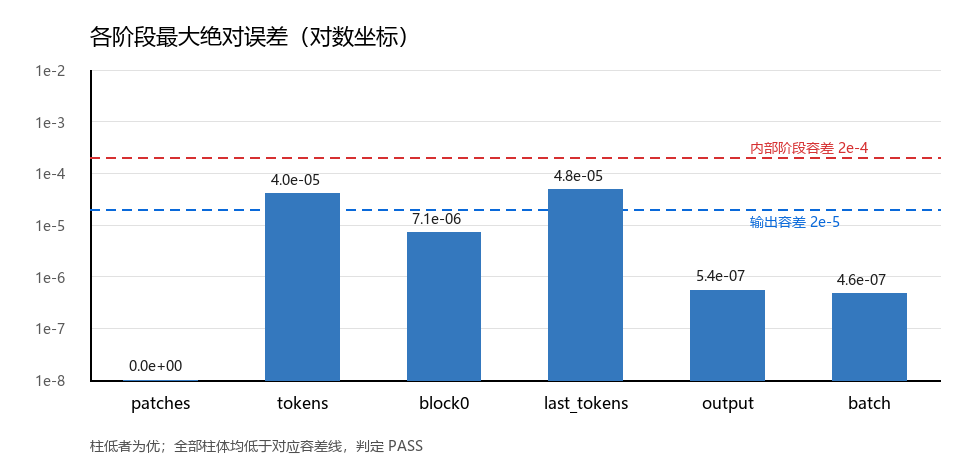
\includegraphics[width=0.8\linewidth]{figs/stage-errors.png}
    \caption{各阶段最大绝对误差（对数坐标）与容差线，所有柱体均低于对应容差}
    \label{fig:err}
\end{figure}

\begin{figure}[H]
    \centering
    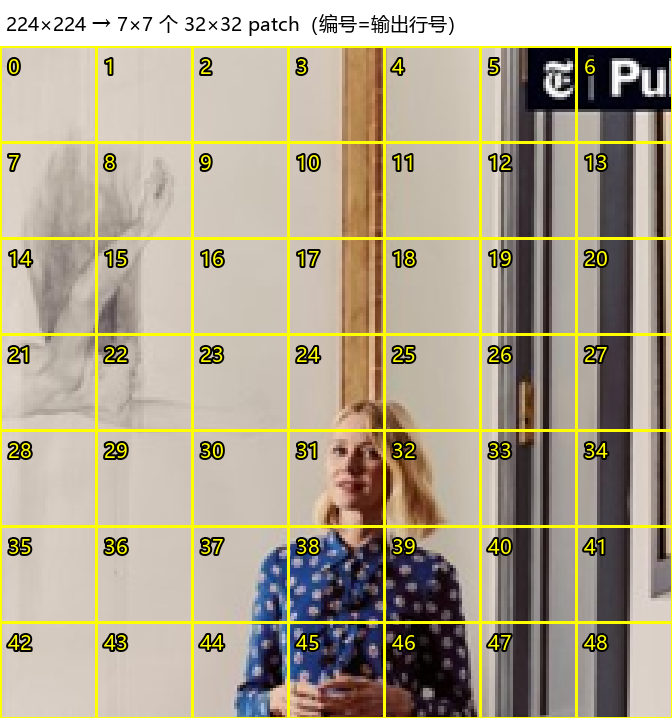
\includegraphics[width=0.46\linewidth]{figs/patch-order.png}
    \caption{49 个 patch 的编号顺序（编号即输出行号），块内按 $C,H,W$ 展平}
    \label{fig:patches}
\end{figure}

图~\ref{fig:patches} 把 image\_01 的 $224\times224$ 输入叠上 $7\times7$ 网格并标注 0--48 的编号，可以直观看到编号沿「先左右、后上下」递增，且与位置编码的顺序一致：一旦这里错位，block0 的误差会立刻升到 $10^{-1}$ 量级（见表~\ref{tab:ablation} 中漏加位置编码一组）。复现全部证据的命令是 \texttt{python check.py --stage all} 与 \texttt{python tools/report\_metrics.py}，后者负责生成表~\ref{tab:errors}、图~\ref{fig:err} 与表~\ref{tab:ablation} 中的每一个数值。

除逐元素误差外还检查了三条可复用性证据：输出每行的 L2 范数为 $1.000000\pm7\times10^{-8}$；10 张图两两余弦相似度为 0.462--0.674，既非特征塌缩也非随机输出；批次按 $[1,0,1]$ 重排（含重复图）与逐张推理的最大差仅 $4.5\times10^{-7}$。这说明实现不依赖缓存或参考行，可处理任意图片与批量，10 张图整条前向耗时 3.2 秒（纯 CPU，单张约 0.3 秒）。

\section{Discussion}

\paragraph{一个形状变化的完整解释}
patchify 是唯一一次连续三步变换：先 reshape 成 $[B,C,7,32,7,32]$，把 $H$、$W$ 各拆成「块位置 + 块内像素」；再 transpose 成「图像、块行、块列、$C$、块内行、块内列」，这一步同时决定 49 行的编号顺序与每个 patch 内部 3072 维的展平顺序，任一写反都仍然合法但数值全错；最后合并成 $[B,49,3072]$。由于转置后内存不连续，必须先 \texttt{ascontiguousarray} 再 reshape，否则 NumPy 会按内存顺序而非逻辑顺序展平。实测这一步与参考完全相等，而 tokens 阶段只剩 $4\times10^{-5}$，说明两个顺序同时正确。

\paragraph{一个 bug 的定位与修复}
最初照搬课程二维示例的写法用 \texttt{k.T} 计算 $QK^{\top}$，运行 block0 时抛出 \texttt{ValueError: matmul 的核心维度不匹配（12 与 64）}。原因是 $k$ 的形状为 $[B,12,50,64]$，\texttt{.T} 会反转全部四个轴得到 $[64,50,12,B]$，最后两维变成 $(12,B)$，无法与 $q$ 相乘；更危险的是若批量恰好为 64 则形状「碰巧」合法、代码不报错但结果完全错误。修复方式是只交换最后两轴：\texttt{k.transpose(0,1,3,2)}。定位过程也值得记录：先跑 patches 与 tokens 确认输入侧无误，再单独跑 block0，打印 $q,k,v$ 的形状并断言 scores 为 $(B,H,N,N)$，修复后 block0 最大误差为 $7.1\times10^{-6}$。

\paragraph{对照实验}
为确认「形状正确不等于语义正确」，实现了六个只错一处的变体，与正确实现对比，结果见表~\ref{tab:ablation}。漏转置、漏位置编码这类错误与正确值相差五个数量级，一定会被检查抓住；而按步长交错切头虽然形状完全合法，误差也达 0.87，属于典型的「形状对、语义错」。

\begin{table}[H]
    \centering
    \small
    \begin{tabular}{|p{9.4cm}|p{3.2cm}|}
    \hline
    单一错误（其余部分保持正确） & block0 最大绝对误差 \\
    \hline
    合并头时漏掉转置 & 1.91 \\
    \hline
    输出投影漏掉转置 & 1.88 \\
    \hline
    漏加位置编码 & 1.78 \\
    \hline
    按 64 维步长交错切分头 & 0.87 \\
    \hline
    图像塔误用因果掩码 & 0.44 \\
    \hline
    4D 张量上直接使用 $k^{\top}$ & 运行时报 ValueError \\
    \hline
    \end{tabular}
    \caption{对照实验：正确实现的 block0 最大误差为 $7.1\times10^{-6}$}
    \label{tab:ablation}
\end{table}

\paragraph{关于误差来源}
三个阶段的最大误差并非随层数单调放大：tokens 为 $4.0\times10^{-5}$，单层 block0 只有 $7.1\times10^{-6}$，12 层叠加后回到 $4.8\times10^{-5}$，最终输出又收缩到 $5.4\times10^{-7}$。这种「不放大」的形态说明差异来自矩阵乘法的累加顺序与分块方式，而非某个轴写反之类的系统性错误——后者会像表~\ref{tab:ablation} 那样直接跳到 $10^{-1}$ 量级。因此把容差继续收紧到 $10^{-7}$ 并无意义，反而会掩盖真实错误。

\paragraph{局限与改进}
其一，课程提供的 GELU 是逐元素 Python 循环调用 math.erf（每层 $B\times50\times3072$ 次），占整条管线绝大部分耗时，改用向量化 erf 可提速 5--10 倍且保持精度，而 tanh 近似会引入约 $10^{-3}$ 的误差，直接超出容差；其二，输入固定为 $224\times224$、patch 固定 32，未支持任意分辨率；其三，与 Torch 约 $10^{-5}$ 的差异来自 BLAS 累加顺序与矩阵乘分块，属 float32 固有，不应盲目追求零误差；其四，目前缺少对 $B=1$、全 0/全 255 极端像素的单元测试，后续可补参数化测试。

\paragraph{反思}
最大的收获是建立「轴语义」的习惯：每次 reshape 或 transpose 都要能说清每个轴代表什么（$B$、token、head、head\_dim、$C$、$h$、$w$）。调试策略上，从第一个出现差异的阶段入手远比逐行读代码高效：patch 精确为 0 排除了索引问题，tokens 只剩 $4\times10^{-5}$ 说明只有浮点差异，问题必然在 block 之后。对 AI 辅助的边界也有了体会：助手能快速给出候选实现与解释，但「这个轴序为什么对」「这个 $10^{-5}$ 是否可以接受」必须自己用数据判断，否则容易把形状对、数值错的代码当成完成。

\newpage

% ============================================================
% 批阅与成绩评定页
% ============================================================

% 绘制正文外框（包含批阅区域）
\begin{tikzpicture}[remember picture, overlay]
  \draw[thick] 
    ($(current page.north west)+(2cm,-3cm)$) 
    rectangle 
    ($(current page.south east)+(-2cm,3.5cm)$);
\end{tikzpicture}

\vspace{1cm}

% 批阅区
\noindent \textbf{指导教师批阅意见：}
\vspace{6cm}
\hfill

\vspace{1cm}

\noindent \textbf{成绩评定：}
\vspace{2cm}
\hfill

\vspace{1cm}

\noindent
\hfill
\textbf{指导教师签字：}\quad\quad\quad\quad\quad\\[0.5cm]

\hfill
\textbf{年}\quad\quad
\textbf{月}\quad\quad
\textbf{日}\quad

\vspace{1cm}

% 备注部分
\noindent \textbf{备注：}

% 框外的注释
\begin{tikzpicture}[remember picture, overlay]
  \node[
    anchor=north west,
    inner sep=0pt,
    text width=\dimexpr\paperwidth-4cm\relax
  ] at ($(current page.south west)+(2cm,3.1cm)$) {
    \begin{minipage}{\dimexpr\paperwidth-4cm\relax}
      \small
      \noindent
      \textbf{注：}\;1、报告内的项目或内容设置，可根据实际情况加以调整和补充。\\[0.2cm]
      \phantom{\textbf{注：}\;}2、教师批改学生实验报告时间应在学生提交实验报告时间后 10 日内。
    \end{minipage}
  };
\end{tikzpicture}

% ============================================================
%                      文档结束
% ============================================================

\end{document}
